\documentclass[a4j]{jarticle}
%%  packages
\usepackage{amsmath,amssymb,ascmac}
\usepackage{bm}
\usepackage[dvipdfmx]{graphicx}
\usepackage{listings}
\usepackage[english]{babel}
\lstset{
 	%枠外に行った時の自動改行
 	breaklines = true,
 	%標準の書体
        basicstyle=\ttfamily\footnotesize,
        commentstyle=\footnotesize\bfseries,
        keywordstyle=\footnotesize\bfseries,
 	%枠 "t"は上に線を記載, "T"は上に二重線を記載
	%他オプション:leftline,topline,bottomline,lines,single,shadowbox
 	frame = single,
 	%frameまでの間隔(行番号とプログラムの間)
 	framesep = 5pt,
 	%行番号の位置
 	numbers = left,
	%行番号の間隔
 	stepnumber = 1,
	%タブの大きさ
 	tabsize = 4,
 	%キャプションの場所("tb"ならば上下両方に記載)
 	captionpos = t
}

%% math commands
\let \ds \displaystyle
\newcommand{\idiff}[3]{
  \frac{d^{#1} #2}{d #3^{#1}}
}
\newcommand{\diff}[3]{
  \frac{\mathrm{d}^{#1} #2}{\mathrm{d} #3^{#1}}
}
\newcommand{\pdiff}[3]{
  \frac{\partial^{#1} #2}{\partial #3^{#1}}
}



%% title configuration
\title{統計的機械学習 ID:05}
\author{05-161026 平出一郎}
\date{\today}


%% headings
\pagestyle{headings}
\markright{統計的機械学習 ID:05}




\begin{document}
%%  begin title page
\thispagestyle{empty}
\maketitle
\pagebreak

\begin{align*}
\int q_{t-1}(z_2)\log p( z_1,z_2 | \bm{\mu},\Sigma) dz_2 &= const - \frac{1}{2}\int q_{t-1}(z_2)\left\{ \Lambda_{11}(z_1-\mu_1)^2 \right. \\
&\quad\quad\quad\quad\quad\quad\quad\quad \left. + 2\Lambda_{12}(z_1-\mu_1)(z_2-\mu_2) +\Lambda_{22}(z_2-\mu_2) \right\} dz_2 \\
&=const' - \frac{1}{2} \left\{ \Lambda_{11}\left(\int q_{t-1}(z_2)dz_2\right)(z_1-\mu_1)^2\right.\\
&\quad\quad\quad\quad\quad\quad\quad\quad \left.+2\Lambda_{12}\left(\int q_{t-1}(z_2)z_2dz_2 - \mu_2 \right)(z_1-\mu_1) \right\} \\
&=const'' - \frac{1}{2}\left\{ z_1-\mu_1+\Lambda_{11}^{-1}\Lambda_{12} \left( \int q_{t-1}(z_2)z_2dz_2 - \mu_2  \right) \right\}^2
\end{align*}


よって$q_t(z_1) = \mathcal{N} ( z_1 | \mu_1- \Lambda_{11}^{-1}\Lambda_{12} ( \int q_{t-1}(z_2)z_2dz_2 - \mu_2) ,\Lambda_{11}^{-1} ) $となる。


同様に$q_t(z_2) = \mathcal{N} ( z_2 | \mu_2- \Lambda_{22}^{-1}\Lambda_{12} ( \int q_{t}(z_1)z_1dz_1 - \mu_1 ) ,\Lambda_{22}^{-1}  )$も成り立つ。

$q_t(z_1) = \mathcal{N}(z_1 |  m^{(t)}_1 \Lambda_{11}^{-1} )$,$q_t(z_2) = \mathcal{N}(z_2 |  m^{(t)}_2 \Lambda_{22}^{-1} )$と書けば,更新式は次のようになる。

$m^{(t)}_1 \leftarrow \mu_1-\Lambda_{11}^{-1}\Lambda_{12} ( m_2^{(t-1)} - \mu_2)$


$m^{(t)}_2 \leftarrow \mu_2-\Lambda_{22}^{-1}\Lambda_{12} ( m_1^{(t)} - \mu_1)$



ランダムに生成したいくつかの$\mu,\Sigma$に対して収束するまで繰り返した。

本来の2変数ガウス分布が細長いときに中心付近に集中した裾野の小さい分布が推論されるのが特徴的である。

結果(複数の初期値に対して。上が本来の分布で下が推論結果の分布)

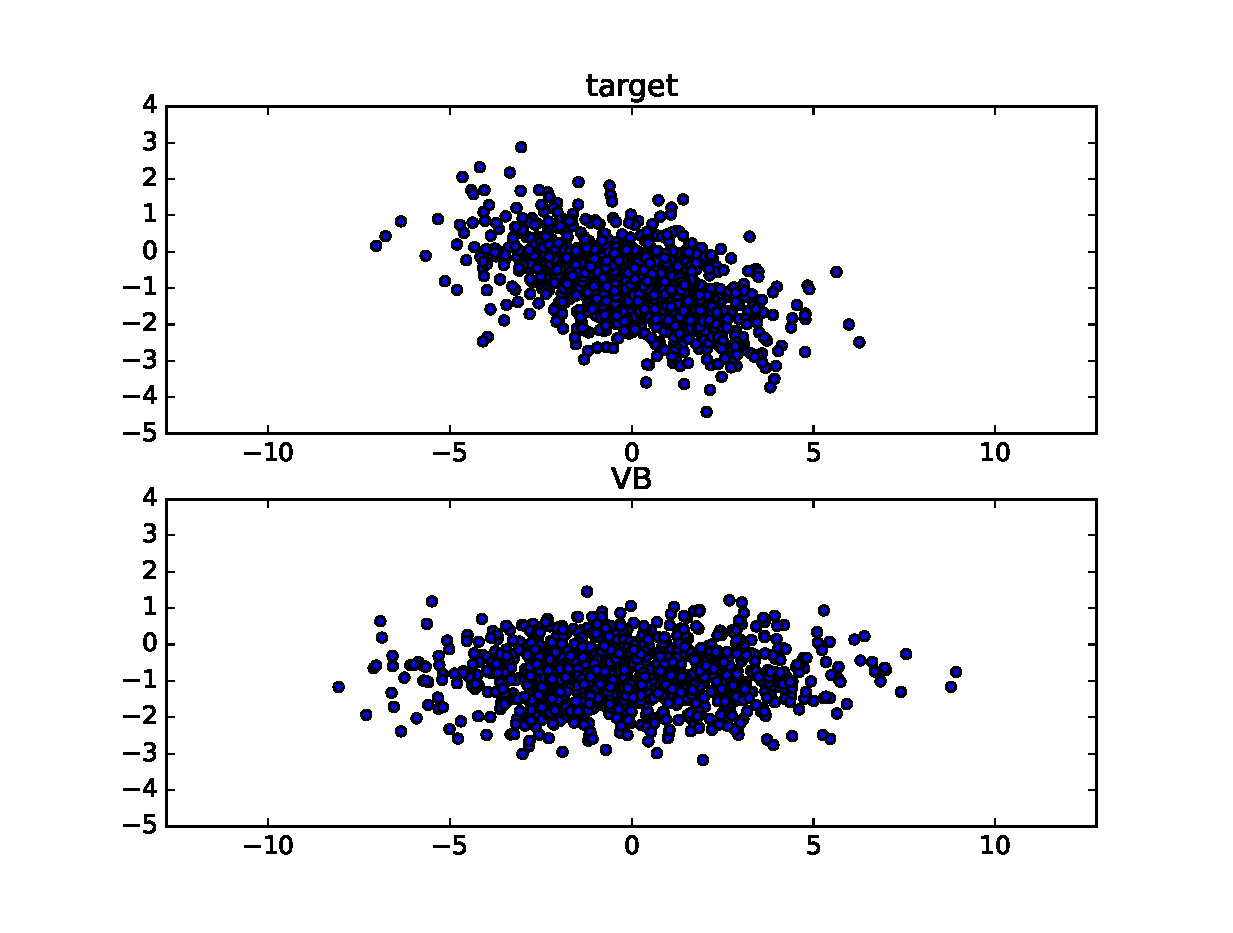
\includegraphics[width=7cm]{fig_1.eps}
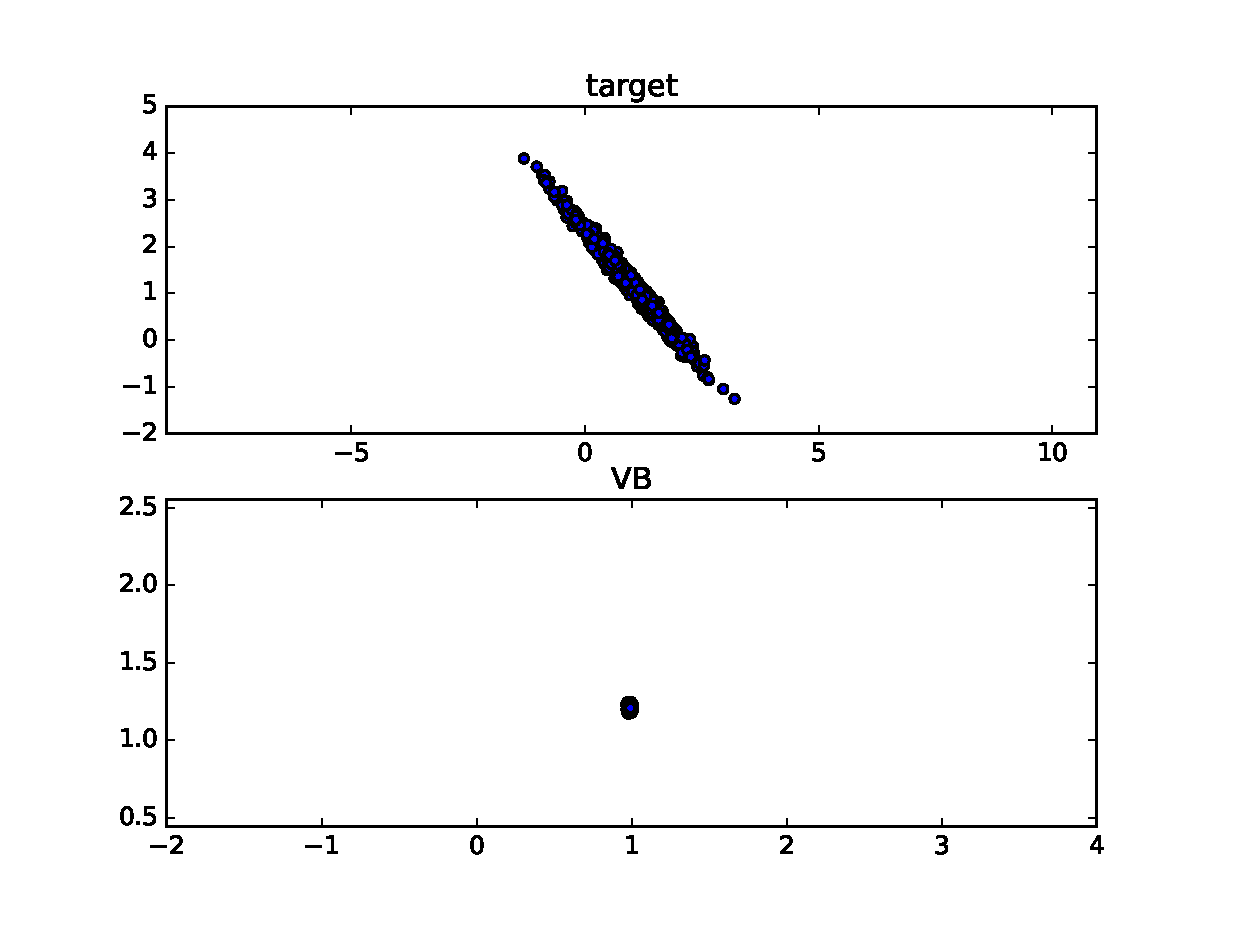
\includegraphics[width=7cm]{fig_2.eps}

\lstinputlisting[caption=source code(Python)]{05.py}

\end{document}


